\chapter{时间信息增强的视觉目标跟踪算法研究}\label{chap:end}
上一章主要研究了如何为基于孪生网络的视觉目标跟踪算法提供更丰富的空间信息以克服跟踪的累计误差。然而,如何在基于孪生网络的视觉目标跟踪算法中利用\textbf{时间信息}尚未得到广泛研究。本章旨在提出一种新型孪生跟踪体系结构,配备有一个时间聚合模块,该模块通过聚合来自相邻帧的时间信息来改善每帧的特征。这种时间聚合策略使孪生跟踪器可以处理由于运动模糊等原因导致的目标表观信息退化现象。此外,本章在孪生网络中整合了对抗性 Dropout 模块,以端到端的方式学习更具判别性的目标特征。本章通过在 GOT-10k \cite{GOT-10k} 和 UAV20L \cite{mueller2016benchmark} 数据集上的大量实验结果,证明了所提出的时间信息增强的视觉目标跟踪算法的有效性。

\section{引言}
视觉目标跟踪的目的是在视频序列每一帧中估计任意目标的状态。 
最近,孪生网络已经为目标跟踪的性能带来显著提高。然而,由于运动模糊等原因导致的目标表观信息退化(图 \ref{fig:end_vis}),往往造成学习到的通用特征表示的判别力下降。
研究人员尝试了不同的方法来改进特征表示。
例如,
%RASNet \cite{wang2018learning} explores diverse attention mechanisms to adapt the offline learned feature representations to a specific tracking target.
SA-Siam \cite{he2018twofold} 分别训练两个分支,以保持语义特征和表观特征的异构性。
在 DaSiamRPN~\cite{zhu2018distractor} 中,作者设计了一个可感知近似物体的增量学习模块,该模块可以有效地将通用嵌入特征迁移到当前视频域,并在推理过程中增量捕获目标表观变化。
SiamRPN++~\cite{SiamRPN++} 引入了一种简单而有效的采样策略,以更强大的深度架构来驱动孪生跟踪器。
上述方法从不同的角度改善了目标的特征表示,并提高了视觉目标跟踪算法的性能。
%These improvements are useful.
%However, all these effort ignores a important problem: they ignore to merge the inter-frame feature during the training phase.
%One important solution is use the temporal information.
%The use of temporal information is important because, when one frame is bad, the adjusting frame can be used. While several method trying to use the temporal information, the method is naive.
%(The bug is, I cannot find any temporal information used in siamese trackers. (I cannot believe it!!! Check it again.--Checked)) For example, A use a time memory to store the appearance information. B use a simple feature average during test. C use history positional information to predict the object position in current frame. However, all these method cannot handle the temporal information during training, which lead to sub-optimal result. To solve this problem, 
然而,这些方法仅利用从当前帧裁剪的特征执行跟踪,这限制了孪生跟踪器的性能。

实际上,视频具有关于目标的丰富信息,并且这种时间信息是视频理解和跟踪的重要基础。
例如,在视频目标检测中,FGFA~\cite{zhu2017flow} 在特征级别上利用了时间一致性。该算法通过沿运动路径聚合相邻帧的特征来改善每帧特征,从而提高了视频识别精度。
在视频目标分割中,STCNN~\cite{xu2019spatiotemporal} 引入了时间模块,该模块着重于捕获动态表观和运动线索以提供目标分割的指导信息。
在基于判别性相关滤波器的目标跟踪中,FlowTrack~\cite{FlowTrack} 专注于利用连续帧中丰富的流信息来改善特征表示和跟踪精度。
但是,如何在孪生跟踪器中利用时间信息尚未得到广泛研究。

\begin{figure*}[t]
    \centering
    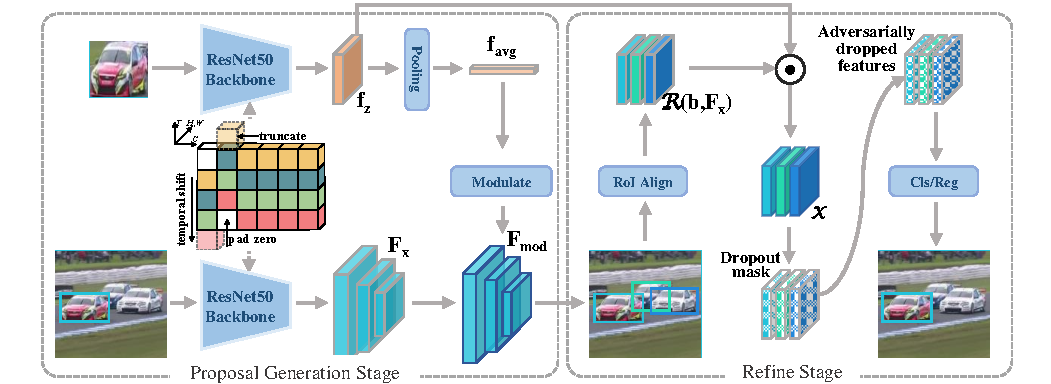
\includegraphics[width=1.0\textwidth]{Img/end/net_v3.pdf}
    \caption{
    本章提出的两阶段跟踪算法框架。
    %At the first stage, a siamese FPN equipped with a temporal aggregation module provides features of the template image and the search image. Then the feature modulation module is used to merge the features and generate proposals.
    %proposals of the object given in the first-frame bounding box. 
    %At the second stage, 
    候选生成阶段旨在生成视觉表观上类似于给定模板目标的候选目标区域。细化阶段旨在从候选目标区域中选择目标。}
    \label{fig:SiamTFA}
\end{figure*}

本章旨在充分利用孪生跟踪器中的时间信息,提出了一种新型孪生跟踪架构,配备有时间聚合模块,该模块通过聚合相邻帧中的特征来改善每帧中目标的特征表示。
这种时间聚合策略使孪生跟踪器可以处理由于运动模糊等原因导致的目标表观信息退化现象。
为实现聚合时间信息的目的,在孪生网络的特征提取网络中沿时间维度 \cite{lin2019tsm} 移动通道特征。
请注意,由于视频中目标的运动 \cite{zhu2017flow},相邻帧中同一目标的特征通常不会在空间上对齐,因此仅对残差层 \cite{lin2019tsm} 进行时间平移,以保证孪生跟踪器的特征学习能力。
与其他时间融合方法 \cite{tao2016siamese, gladh2016deep} 不同,本章采用的方法能够在大规模数据集上进行端到端训练。此外,本章采用的时间融合方法易于实现,而无需更改孪生跟踪架构或使用光流 \cite{FlowTrack} 信息。

为了提高目标特征的鲁棒性,本章在孪生跟踪网络中进一步整合了一个对抗性 Dropout \cite{park2018adversarial} 模块。
具体而言,首先根据散度最大化预测对抗性 Dropout 模板。
然后,最大程度地减小随机删除的特征和对抗删除的特征之间的差异。
该模块具有 Dropout 和对抗训练的双重优势:Dropout 使基于孪生网络的视觉目标跟踪器在训练过程中随机断开神经元,以防止目标特征的过拟合;而对抗训练则使基于孪生网络的视觉目标跟踪器学习困难的情况。

总体来说,本章的贡献有三个方面:
\begin{itemize}
\item 本章提出了一种新型孪生跟踪体系结构,配备有时间聚合模块,可通过聚合相邻帧的特征来改善每帧中目标的特征表示。
\item 本章在孪生网络跟踪器中进一步引入了对抗性 Dropout 模块,以提高孪生跟踪网络的特征判别能力。
\item 在 GOT-10k \cite{GOT-10k} 和 UAV20L \cite{mueller2016benchmark} 跟踪数据集上的大量实验结果,证明了基于时间信息增强的跟踪系统的有效性(图 \ref{fig:end_vis})。
\end{itemize}

\section{相关工作}
\subsection{时间信息在视频动作识别中的应用}
远程时间结构在理解动作视频的动态过程中起着重要的作用。但是,主流的卷积神经网络框架通常集中在表观信息和短期运动上,因此缺乏整合远程时间结构的能力。最近,有一些尝试 \cite{Motionlets} 来解决这个问题。这些方法主要依赖于具有预定采样间隔的密集时间采样。当将这种方法应用于长视频序列时,将导致过高的计算成本,这限制了其在现实世界中的应用,并存在丢失长视频中重要信息的风险。因此,在 文献 \cite{TSN} 中,Wang 等人基于远程时间结构建模的思想,提出了一种视频动作识别的新型框架。该框架结合了稀疏的时间采样策略和视频级别的监督,可以使用整个动作视频进行高效学习。该框架采用稀疏采样方案在长视频序列上提取短视频片段,其中采样点沿时间维度均匀分布。在此基础上,采用分层结构聚合来自采样视频段的信息。因此,该算法能够对整个视频的远程时间结构进行建模。此外,这种稀疏的采样策略可以使用较低的成本保存视频信息,从而可以在合理的时间和计算资源预算下,在长视频序列上进行端到端学习。% Temporal Segment Networks: Towards Good Practices for Deep Action Recognition 1608
在文献 \cite{TRN} 中,Zhou 等人认为时间关系推理使人类能够根据过去情况分析当前情况,并就下一步可能发生的情况提出假设。时间关系推理对于视频动作识别至关重要,它构成了描述事件的基础。因此,作者提出了一种有效且可解释的网络模块,即时间关系网络(temporal relational reasoning,TRN),该模块旨在学习和推理多个时间尺度上视频帧之间的时间依赖性。% Temporal Relational Reasoning in Videos 1711
在文献 \cite{AdaFuse} 中,Meng 等人认为时间建模是有效的视频动作识别的关键。虽然了解时间信息可以提高动态动作的识别精度,但是消除时间冗余和重用过去的特征可以大大节省计算量,从而实现有效的动作识别。因此,作者提出了一种称为 AdaFuse 的自适应时间融合网络,该网络可以动态融合当前和过去特征图中的通道,以实现强大的时间建模,从而提高识别精度和效率。% ADAFUSE: ADAPTIVE TEMPORAL FUSION NETWORK FOR EFFICIENT ACTION RECOGNITION
\subsection{时间信息在视频目标检测中的应用}
在视频目标检测算法 TCNN \cite{TCNN} 中,Kang 等人认为在相邻帧中目标的位置和表观应保持连续性,即,预测的边界框位置和检测置信度不应在短时间内发生剧烈变化。然而,如果将图像目标检测框架直接应用于视频目标检测任务中,则目标的检测置信度往往会在相邻帧之间发生显著变化。为了解决这一问题,作者提出了一个深度学习框架,该框架扩展了流行的图像检测框架 R-CNN \cite{girshick2014rich} 和 Faster R-CNN \cite{ren2015faster},通过合并相邻帧的时间信息和上下文信息来解决视频中的通用目标检测问题。该算法可以在相邻帧中传播检测结果,并可沿着跟踪算法生成的轨迹修改检测置信度,从而有效地提高现有图像检测框架在视频目标检测任务中的性能。% T-CNN: Tubelets with Convolutional Neural Networks for Object Detection from Videos 1604
该工作虽然提高了识别准确性,但是具有较高的计算成本。为了减少计算量,在文献 \cite{DeepFeature} 中,Zhu 等人基于深度特征流提出了一种快速、准确的视频目标检测方法。该方法在稀疏的关键帧上应用图像检测网络,通过流场将深度特征图从关键帧传播到其他帧。传播后的特征类似于原始特征。通常,流估计和特征传播比卷积特征的计算快得多。因此,该方法避免了计算瓶颈,显著提高了检测速度。当流场也由网络估算时,整个架构将进行端到端训练,可同时优化目标检测任务和流网络。% Deep Feature Flow for Video Recognition
\subsection{时间信息在视觉目标跟踪中的应用}
大多数现有的相关滤波跟踪器仅考虑当前帧的表观特征,几乎无法从运动和帧间信息中受益。在诸如部分遮挡和形变之类的挑战中,缺少时间信息会降低跟踪性能。目标跟踪所处理的是视频信息,因此时序信息很重要。
%以前有很多工作利用时序信息进行目标跟踪。
在文献 \cite{gladh2016deep} 中,Gladh 等人首次提出将表观信息与深度运动特征融合以进行视觉跟踪。表观特征仅对单帧中的静态信息进行编码,而深度运动特征则对基于光流的多帧信息进行整合。因此,运动特征可以捕获与表观特征互补的场景动态特征。因此,作者研究了深度运动特征对视觉目标跟踪的影响,并提出将表观特征与深度运动特征进行融合,以进行视觉目标跟踪。
该方法虽然利用光流提高了视觉目标跟踪算法的性能,但采用的是在动作识别任务中预训练的深层光流网络,并没有在视觉目标跟踪任务中进行端到端训练,因此没有获得最佳跟踪效果。
为了解决这一问题,FlowTrack \cite{FlowTrack} 首次提出在深度学习框架中共同训练光流网络和跟踪网络,从而利用连续帧中丰富的光流信息进一步提高特征表示和跟踪精度。首先,作者将包括光流估计、特征提取、特征聚合和相关滤波器跟踪在内的各个组件制定为网络中的特殊层。然后,按照光流的引导,以指定的时间间隔对历史特征图进行扭曲并与当前特征图进行聚合,从而捕获视频中的时间信息。

\section{孪生网络跟踪器的端到端时间聚合}
本文提出的跟踪网络(图 \ref{fig:SiamTFA})基于孪生跟踪架构 \cite{SiamRPN++, Wang2018SiamMask},将图像对作为输入,包括模板图像和搜索图像。模板图像是根据真实边界框从初始帧裁剪的图像块。搜索图像是视频序列中的某一帧。两个输入共享相同的特征提取器和网络参数。
受两阶段检测框架 \cite{ren2015faster} 启发,本章提出的孪生跟踪器也是一种两阶段方法。第一阶段旨在生成在视觉上类似于给定模板目标的候选目标区域。在该阶段,引入一个时间聚合模块以增强时间信息(第 \ref{sec:stage1} 节)。第二阶段旨在从候选目标区域中确定跟踪的最终结果。在该阶段,引入一个对抗性 Dropout 模块以学习更具判别性的特征(第 \ref{sec:stage2}节)。

\subsection{时间聚合模块}
\label{sec:stage1}
候选目标生成阶段包括三个组件:(1)特征提取器,(2)时间聚合模块和(3)特征调制模块。
特征提取器分别为搜索图像和模板图像生成搜索特征和模板特征。时间聚合模块被集成到特征提取器中以利用时间信息。特征调制模块聚合搜索特征和模板特征以识别候选目标。

\textbf{特征提取器} 为了处理目标的尺度变化,本章使用 ResNet50-FPN \cite{lin2017feature} 作为特征提取器。
\textbf{F}eature \textbf{P}yramid \textbf{N}etwork(FPN)利用深层卷积网络固有的多尺度金字塔层次结构来构建具有较小计算成本的特征金字塔。
特征金字塔是目标检测领域用于检测不同尺度目标的重要组件。
然而传统的特征金字塔方法往往需要消耗大量计算资源和内存空间。为了解决这一问题,FPN 开发了具有横向连接的自上而下的体系结构,以构建各种尺度的高级语义特征图。
FPN 作为通用的特征提取器,为多种计算机视觉应用带来了显著的性能改进。
因此,本章将 FPN 体系结构引入孪生网络跟踪器当中。所提出的孪生 FPN 将模板图像和搜索图像作为输入。对于搜索图像,FPN 以完全卷积的方式在多个级别上输出不同尺度的特征图。
搜索图像的输出特征图表示为 $F_{\textbf x} = \{f_{\textbf x}^i\}_{i=1:5}$,特征图的步幅分别为 \{4, 8, 16, 32, 64\} 像素。
对于模板图像,使用 FPN 最后阶段的输出作为模板特征,其空间大小为 $7 \times 7$。

\textbf{时间聚合模块}
大多数基于孪生网络的视觉目标跟踪算法 \cite{SiamRPN++, Wang2018SiamMask} 使用静止图像预测目标的位置,% However, tracking on single frame generates unstable results and fails when appearance is pool \cite{zhu2017flow}. 
这限制了孪生跟踪器的能力。
一方面,基于单帧进行跟踪可能会产生不稳定的结果,从而导致在目标表观发生退化时跟踪失败(图 \ref{fig:end_vis});另一方面,
在时间上相邻的帧可以提供有关目标的更多信息。
因此,本章旨在通过聚合相邻帧的特征来改善每帧中的目标特征。
相比于三维卷积神经网络,传统的二维卷积神经网络消耗的计算资源相对较少,但无法捕获时间关系。基于三维卷积神经网络的方法可以提取时间维度的特征,但计算量大,因此部署成本高。在本章所设计的跟踪器中,引入了一种性能高、速度快的通用时间移位模块(temporal shift module,TSM)\cite{lin2019tsm}。具体来说,该模块可以实现三维卷积神经网络的性能,同时保持二维卷积神经网络的复杂性。时间移位模块沿时间维度移动部分通道,因此可以在相邻帧之间交换信息。该模块可以直接插入二维卷积神经网络中,在不增加计算量和参数量的情况下实现时间建模。具体来说,神经网络中的特征激活可以表示为 $f \in \mathbb R^{N\times C\times T\times H\times W}$,其中 $N$ 是批次大小,$C$ 是通道数,$T$ 是时间维度,$H$ 和 $W$ 是空间分辨率。传统的二维卷积神经网络在不同的时间 $T$ 上独立运行,因此无法进行时间建模。而时间移位模块沿时间维度向前或向后移动通道,使得来自相邻帧的信息在移位后与当前帧混合在一起。
尽管移位运算不会增加计算量,但仅简单地平移通道信息会带来两个主要的问题:
\begin{itemize}
\item 效率不高:移位运算在理论上不会增加计算量,但会导致数据移动。数据移动的额外成本不可忽略,并且会导致延迟增加。这种现象在占用大量内存空间的视频理解神经网络中更加严重。
\item 准确性差:在网络中移动太多通道会严重损害空间建模能力,并导致性能下降。
\end{itemize}

为了解决这些问题,在文献 \cite{lin2019tsm} 中,Lin 等人提出了两个解决方案:
\begin{itemize}
\item 采用局部移位策略:为了有效的时间融合,只移位一小部分通道,而不是移位所有通道。这种策略显著降低了数据移动成本。
\item 将时间移位模块插入残差分支内,以便保留当前帧的激活,这不会损害二维卷积神经网络的空间特征学习能力。
\end{itemize}

本章提出,将该模块插入到基于孪生网络的视觉目标跟踪算法中。具体来说,将时间聚合模块插入孪生特征提取器的最后一个阶段。
为了对时间信息进行建模,一批图像是同一视频中的几个相邻帧,并按时间排序,因此可以将批次维度视为时间维度。假设特征提取器最后阶段的特征图表示为 $f \in \mathbb R ^ {T \times C \times H \times W}$。
对于时刻 $t \leq T$,首先将特征 $f^t \in \mathbb R ^ {C \times H \times W}$ 沿通道维度分为三部分:$f_{1:K}^t \in \mathbb R ^ {K \times H \times W}$,$f_{(K+1):2K}^t \in \mathbb R ^ {K \times H \times W}$ 和 $f_{(2K+1):C}^t \in \mathbb R ^ {(C-2K) \times H \times W}$。
然后,按照文献 \cite{lin2019tsm} 沿时间维度移动通道:
\begin{equation}
    f_{agg}^t = \mathcal{C}(f_{{1:K}}^{t-1}, f_{(K+1):2K}^{t+1}, f_{(2K+1):C}^{t}),
\end{equation}
其中 $\mathcal{C}(\cdot)$ 是串接操作。根据文献 \cite{lin2019tsm},移位操作仅在残差层执行,以保留孪生跟踪器的空间特征学习能力。
请注意,聚合特征 $f_{agg}^t$ 具有与 $f^t$ 相同的形状,因此可以将此模块直接插入到主干网络中,而无需更改网络的其他部分。
而且,此操作仅需要进行数据移动,并且可以端到端进行训练。

\textbf{特征调制模块} 在获得模板特征 $f_{\textbf z}$ 和搜索图像的特征金字塔 $F_{\textbf x} = \{f_{\textbf x}^i\}_{i=1:5}$ 之后,对其进行调制以生成特定于目标的特征。
具体而言,使用全局平均池化操作根据 $f_{\textbf z}$ 生成调制矢量 $f_{avg}$,该调制矢量携带目标特定的表观信息。
调制后的特征金字塔 $F_{mod} = \{f_{mod}^i\}_{i=1:5}$ 的生成方式如下:
\begin{equation}
    f_{mod}^i = f^i_{\textbf x} \star f_{avg},
\end{equation}
其中 $\star$ 是逐通道互相关操作 \cite{SiamRPN++}。
每个调制后的特征图都被送入两个并行的全连接层中——通道尺寸为 $4k$ 的边框回归层和通道尺寸为 $2k$ 的边框分类层,其中 $k$ 是每个空间位置的最大候选目标数量。
在本章中,根据文献 \cite{lin2017feature} 将具有相同尺度的锚框分配给每个不同的金字塔层级,使用得分最高的前 $N$ 个候选目标区域送入细化阶段进行后处理。

\subsection{对抗性 Dropout 模块}
\label{sec:stage2}
细化阶段旨在从候选目标区域中选择目标。
这些候选目标的特征使用 RoI Align \cite{he2017mask} 操作从搜索特征金字塔 $F_{\textbf x}$ 中裁剪出来,然后与目标特征 $f_{\textbf z}$ 进行融合:
\begin{equation}
    \mathcal{X} = \mathcal{R}(b, F_{\textbf x}) \odot f_{\textbf z},
\end{equation}
其中 $\mathcal{R}$ 表示 RoI Align 操作,$\odot$ 表示逐元素相乘操作,$b$ 表示候选目标区域,$\mathcal{X}$ 表示候选目标区域 $b$ 的融合特征。

\begin{figure}[t]
    \centering
    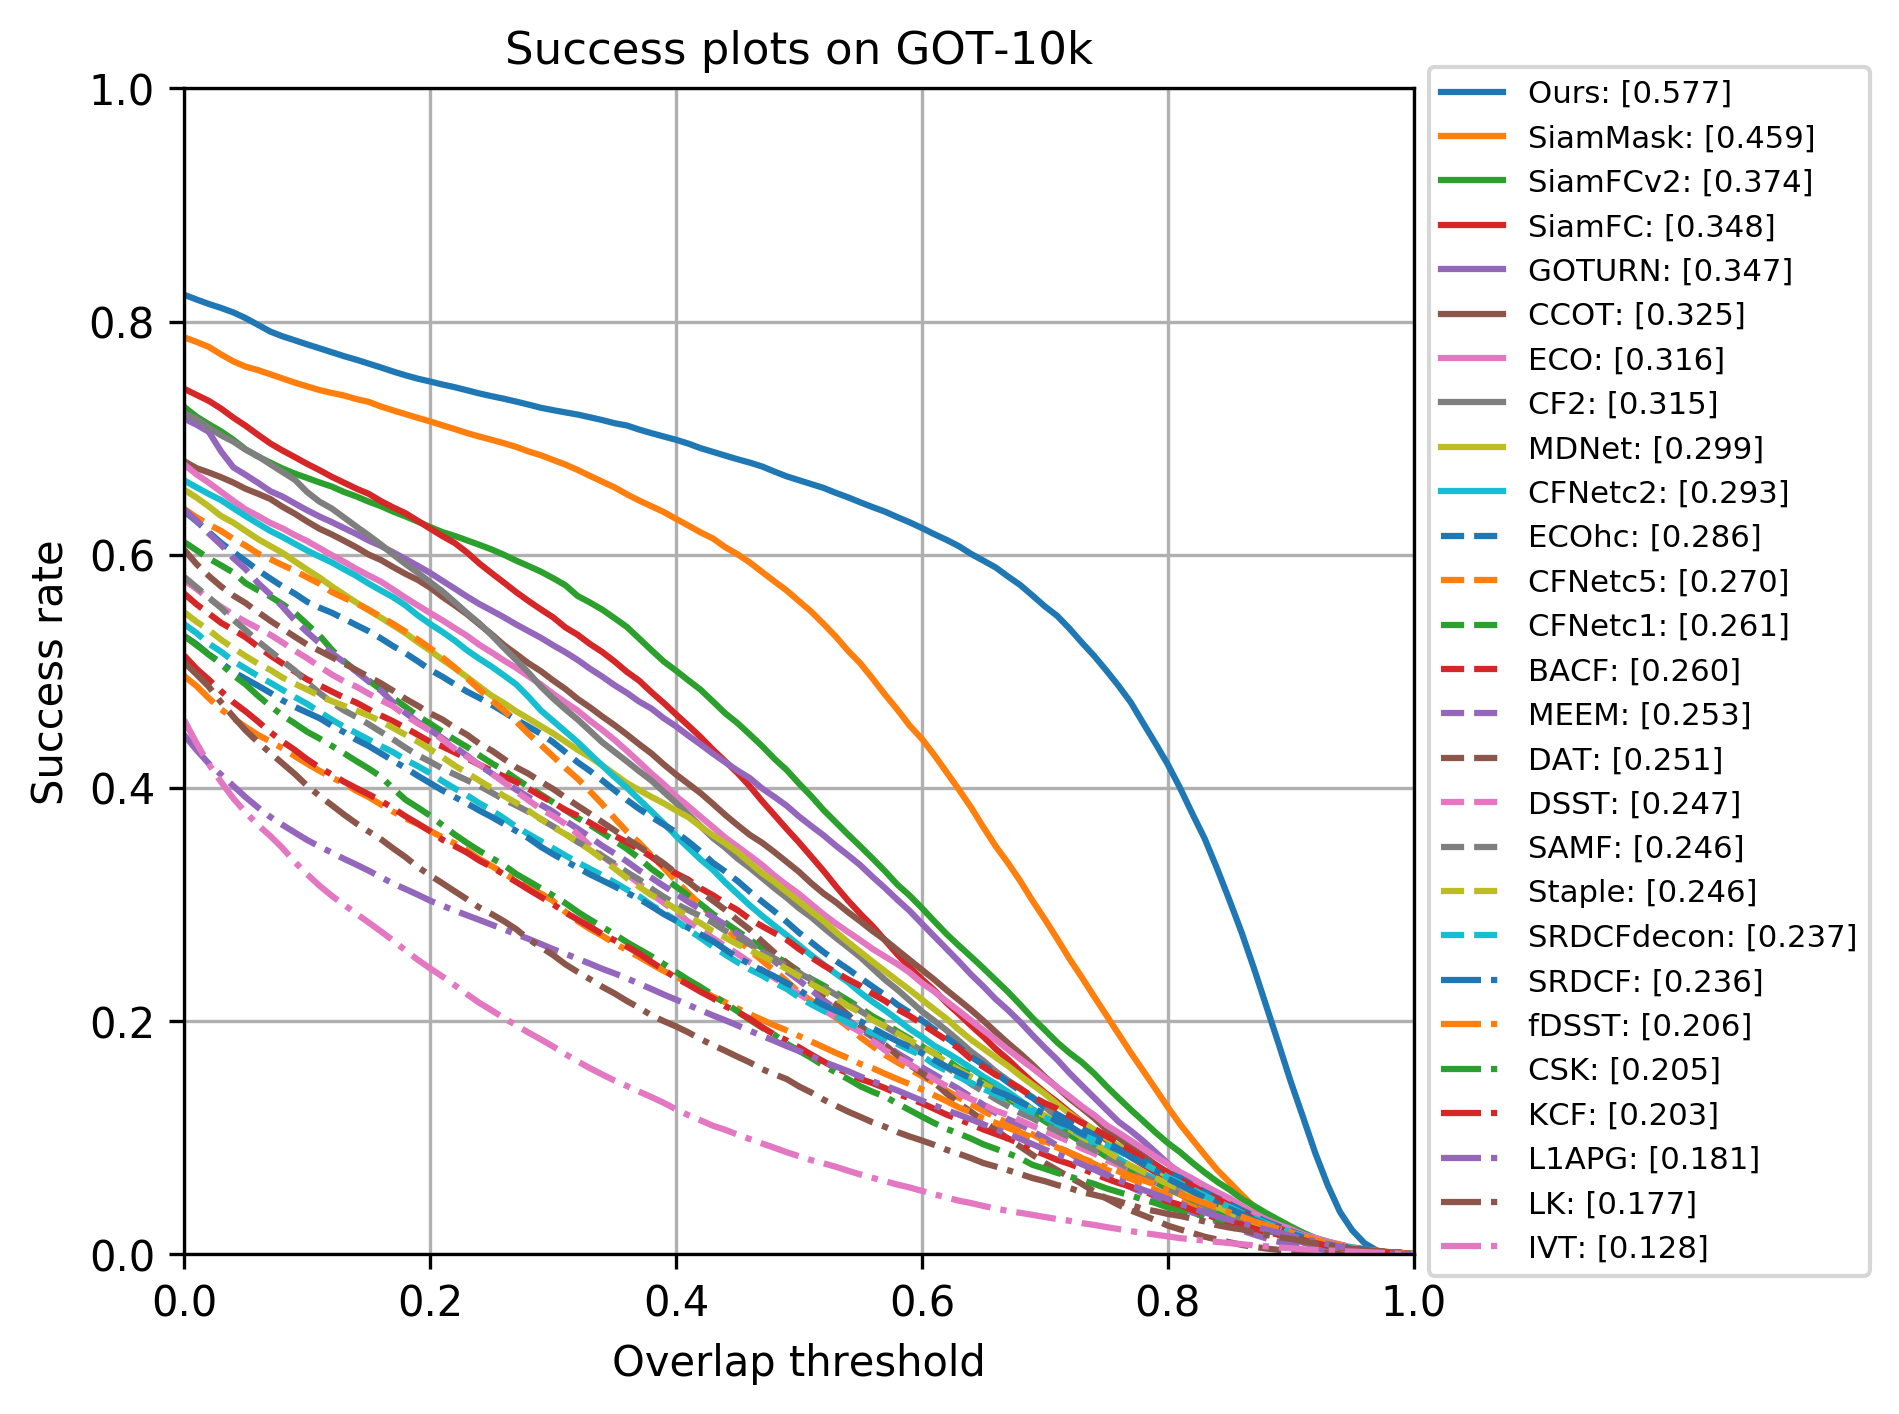
\includegraphics[width=0.75\textwidth]{Img/end/success_plot.png}
    \caption{数据集 GOT-10k \cite{GOT-10k} 中算法的平均重叠率(AO)排序图。}
    \label{fig:end_got10k}
\end{figure}

\textbf{对抗性 Dropout} 特征融合之后,本章算法使用对抗性 Dropout \cite{park2018adversarial, lee2019drop} 来提高 $\mathcal{X}$ 的判别能力。
之所以使用这一模块,是因为 Dropout 是一种简单而有效的正则化方法,可以在训练过程中随机丢弃一部分神经元。Srivastava 等人 \cite{srivastava2014dropout} 指出, Dropout 具有整合网络的多个子集的作用。 Park 等人 \cite{park2016analysis} 着重指出了卷积层上的 Dropout 效果。Tompson 等人 \cite{tompson2015efficient} 指出,卷积层的激活通常被同一特征图中的类似激活所包围;因此,丢弃单个神经元在卷积层中没有强大的作用。取而代之的是,他们提出了空间 Dropout 的方法,即丢弃整个特征图,而不是单个神经元。 Hou 等人 \cite{hou2019weighted} 在空间 Dropout 的基础上,提出了一种加权的通道 Dropout 方案,该方案对各个通道使用可变的丢弃率,其中丢弃率取决于通道的平均激活值。加权通道 Dropout 仅应用于网络的较深层,在这些较深的层中,激活具有很高的特异性。
\begin{figure}[t]
\begin{minipage}{0.48\textwidth}
  \centering
  \centerline{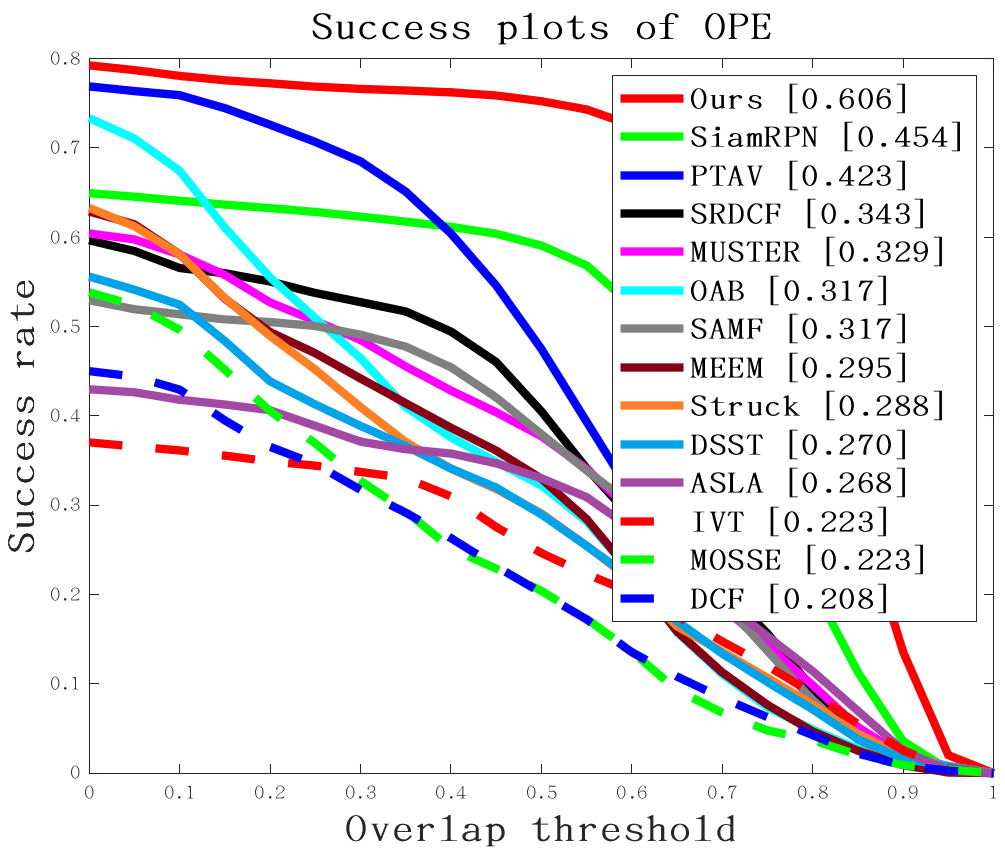
\includegraphics[width=0.99\textwidth]{Img/end/quality_plot_overlap_OPE_AUC.png}}
\end{minipage}
\hfill
\begin{minipage}{0.48\textwidth}
  \centering
  \centerline{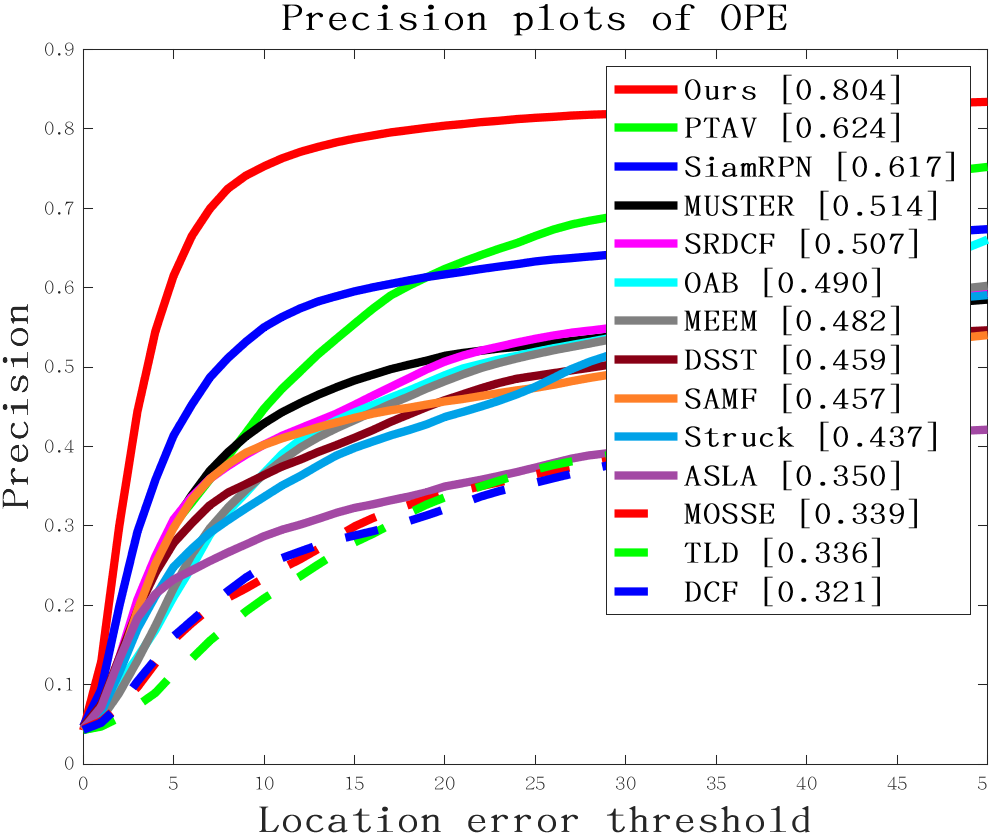
\includegraphics[width=0.99\textwidth]{Img/end/quality_plot_error_OPE_threshold.png}}
\end{minipage}
\caption{本章提出的跟踪算法与相关算法在 UAV20L \cite{mueller2016benchmark} 数据集上的跟踪成功率曲线以及精度曲线展示。}
\label{fig:end_uav20l}
\end{figure}
对抗性 Dropout 是一种用于监督和半监督学习的有效正则化方法。具体来说,Park 等人 \cite{park2018adversarial} 定义了两种类型的对抗性 Dropout:监督对抗性 Dropout(SAdD)和虚拟对抗性 Dropout(VAdD)。如果存在真实标注信息,可以使用 SAdD 最大化模型预测与真实标注信息之间的差异。另一方面,如果没有标签,则使用 VAdD 最大化输入的两个独立预测之间的差异。% Drop to Adapt: Learning Discriminative Features for Unsupervised Domain Adaptation
在本章中,通过引入对抗性 Dropout 以提高被跟踪目标的特征判别性:首先根据散度最大化预测对抗性 Dropout 掩码,将该掩码应用于 $\mathcal{X}$,以获得对抗性 Dropout 的特征;然后,最大程度地减少随机 Dropout 的特征和对抗性 Dropout 的特征之间的差异。
具体而言,令 $h^{cls}$ 和 $h^{reg}$ 分别表示细化阶段中的分类层和回归层。
根据文献 \cite{lee2019drop},按如下方式计算对抗性 Dropout 掩码:
\begin{equation}
\begin{split}
    & \mathbf{m}^{adv} = \mathop{\arg\max}\limits_{\mathbf{m}}D[h^{cls}(\mathcal{X} \odot \mathbf{m}^s), h^{cls}(\mathcal{X} \odot \mathbf{m})] \\
    & ||\mathbf{m}^s - \mathbf{m}|| \leq \delta_e L,
\end{split}
\end{equation}
其中 $L$ 代表 $\mathbf{m} \in \mathbb R^L$ 的尺寸,
$\mathbf{m}^s$ 表示随机 Dropout 掩码, $\mathbf{m}^{adv}$ 表示对抗性 Dropout 掩码。
$\delta_{e}$ 是一个超参数,用于控制相对于 $\mathbf{m}^{s}$ 的扰动幅度 \cite{lee2019drop}。
%and $\delta_{e}$ is a hyper parameter to control the perturbation magnitude with respect to $m^{s}$ \cite{lee2019drop}
$D[p, p'] \geq 0$ 测量两个分布 $p$ 和 $p'$ 之间的差异。

为了计算 $\mathbf{m}^{adv}$,文献 \cite{park2018adversarial} 通过在计算过程中进行适当放松来优化 0/1 背包问题。
在生成 $\mathbf{m}^{adv}$ 之后,最小化 $\mathcal{X}$ 的两个预测分布之间的差异:一个采用随机 Dropout 掩码 $\mathbf{m}^{s}$ 获得,另一个采用对抗性 Dropout 掩码 $\mathbf{m}^{adv}$ 获得 \cite{lee2019drop}:
\begin{equation}
    \mathcal{L}_{adv} = \mathbb E[D_{KL}[h^{cls}(\mathcal{X} \odot\mathbf{m}^{s})||h^{cls}(\mathcal{X} \odot\mathbf{m}^{adv}))]],
\end{equation}
其中 $D_{KL}$ 是 Kullback-Leibler 散度。

最后,对于每个候选目标区域,分类层在两个类别(前景或背景)上生成 softmax 概率估计,而回归层为前景类别输出四个实数值,用于编码候选目标区域的精确边界框位置。
网络的整体损失函数是:
\begin{equation}
\mathcal{L} = \mathcal{L}_{cls}^{stage1} + \mathcal{L}_{cls}^{stage2} + \mathcal{L}_{reg}^{stage1}+\mathcal{L}_{reg}^{stage2} +  \lambda \mathcal{L}_{adv},
\end{equation}
其中 $\lambda$ 是用于平衡对抗损失和分类/回归损失的超参数。$\mathcal{L}_{cls}^{\cdot}$ 是交叉熵损失,$\mathcal{L}_{reg}^{\cdot}$ 是回归分支的平滑 $L1$ 损失。在测试过程中,具有最高分类得分的区域被选择为预测目标。

\begin{table}[t]
\centering
\caption{时间聚合模块以及对抗性 Dropout 模块在 GOT-10k \cite{GOT-10k} 测试集上的有效性展示。}
\begin{tabular}{c c c c c}
\bottomrule
时间聚合模块 & 对抗性 Dropout 模块 & AO & $\text{SR}_{0.50}$ & $\text{SR}_{0.75}$ \\ 
\hline
          &           & 0.542 & 0.607 & 0.456 \\
\checkmark&           & 0.561 & 0.645 & 0.480 \\
\checkmark&\checkmark & 0.577 & 0.662 & 0.509 \\
\bottomrule
\end{tabular}
\label{table:end_ablition}
\end{table}

\section{实验评估与分析}

\begin{figure}[p]
    \centering
    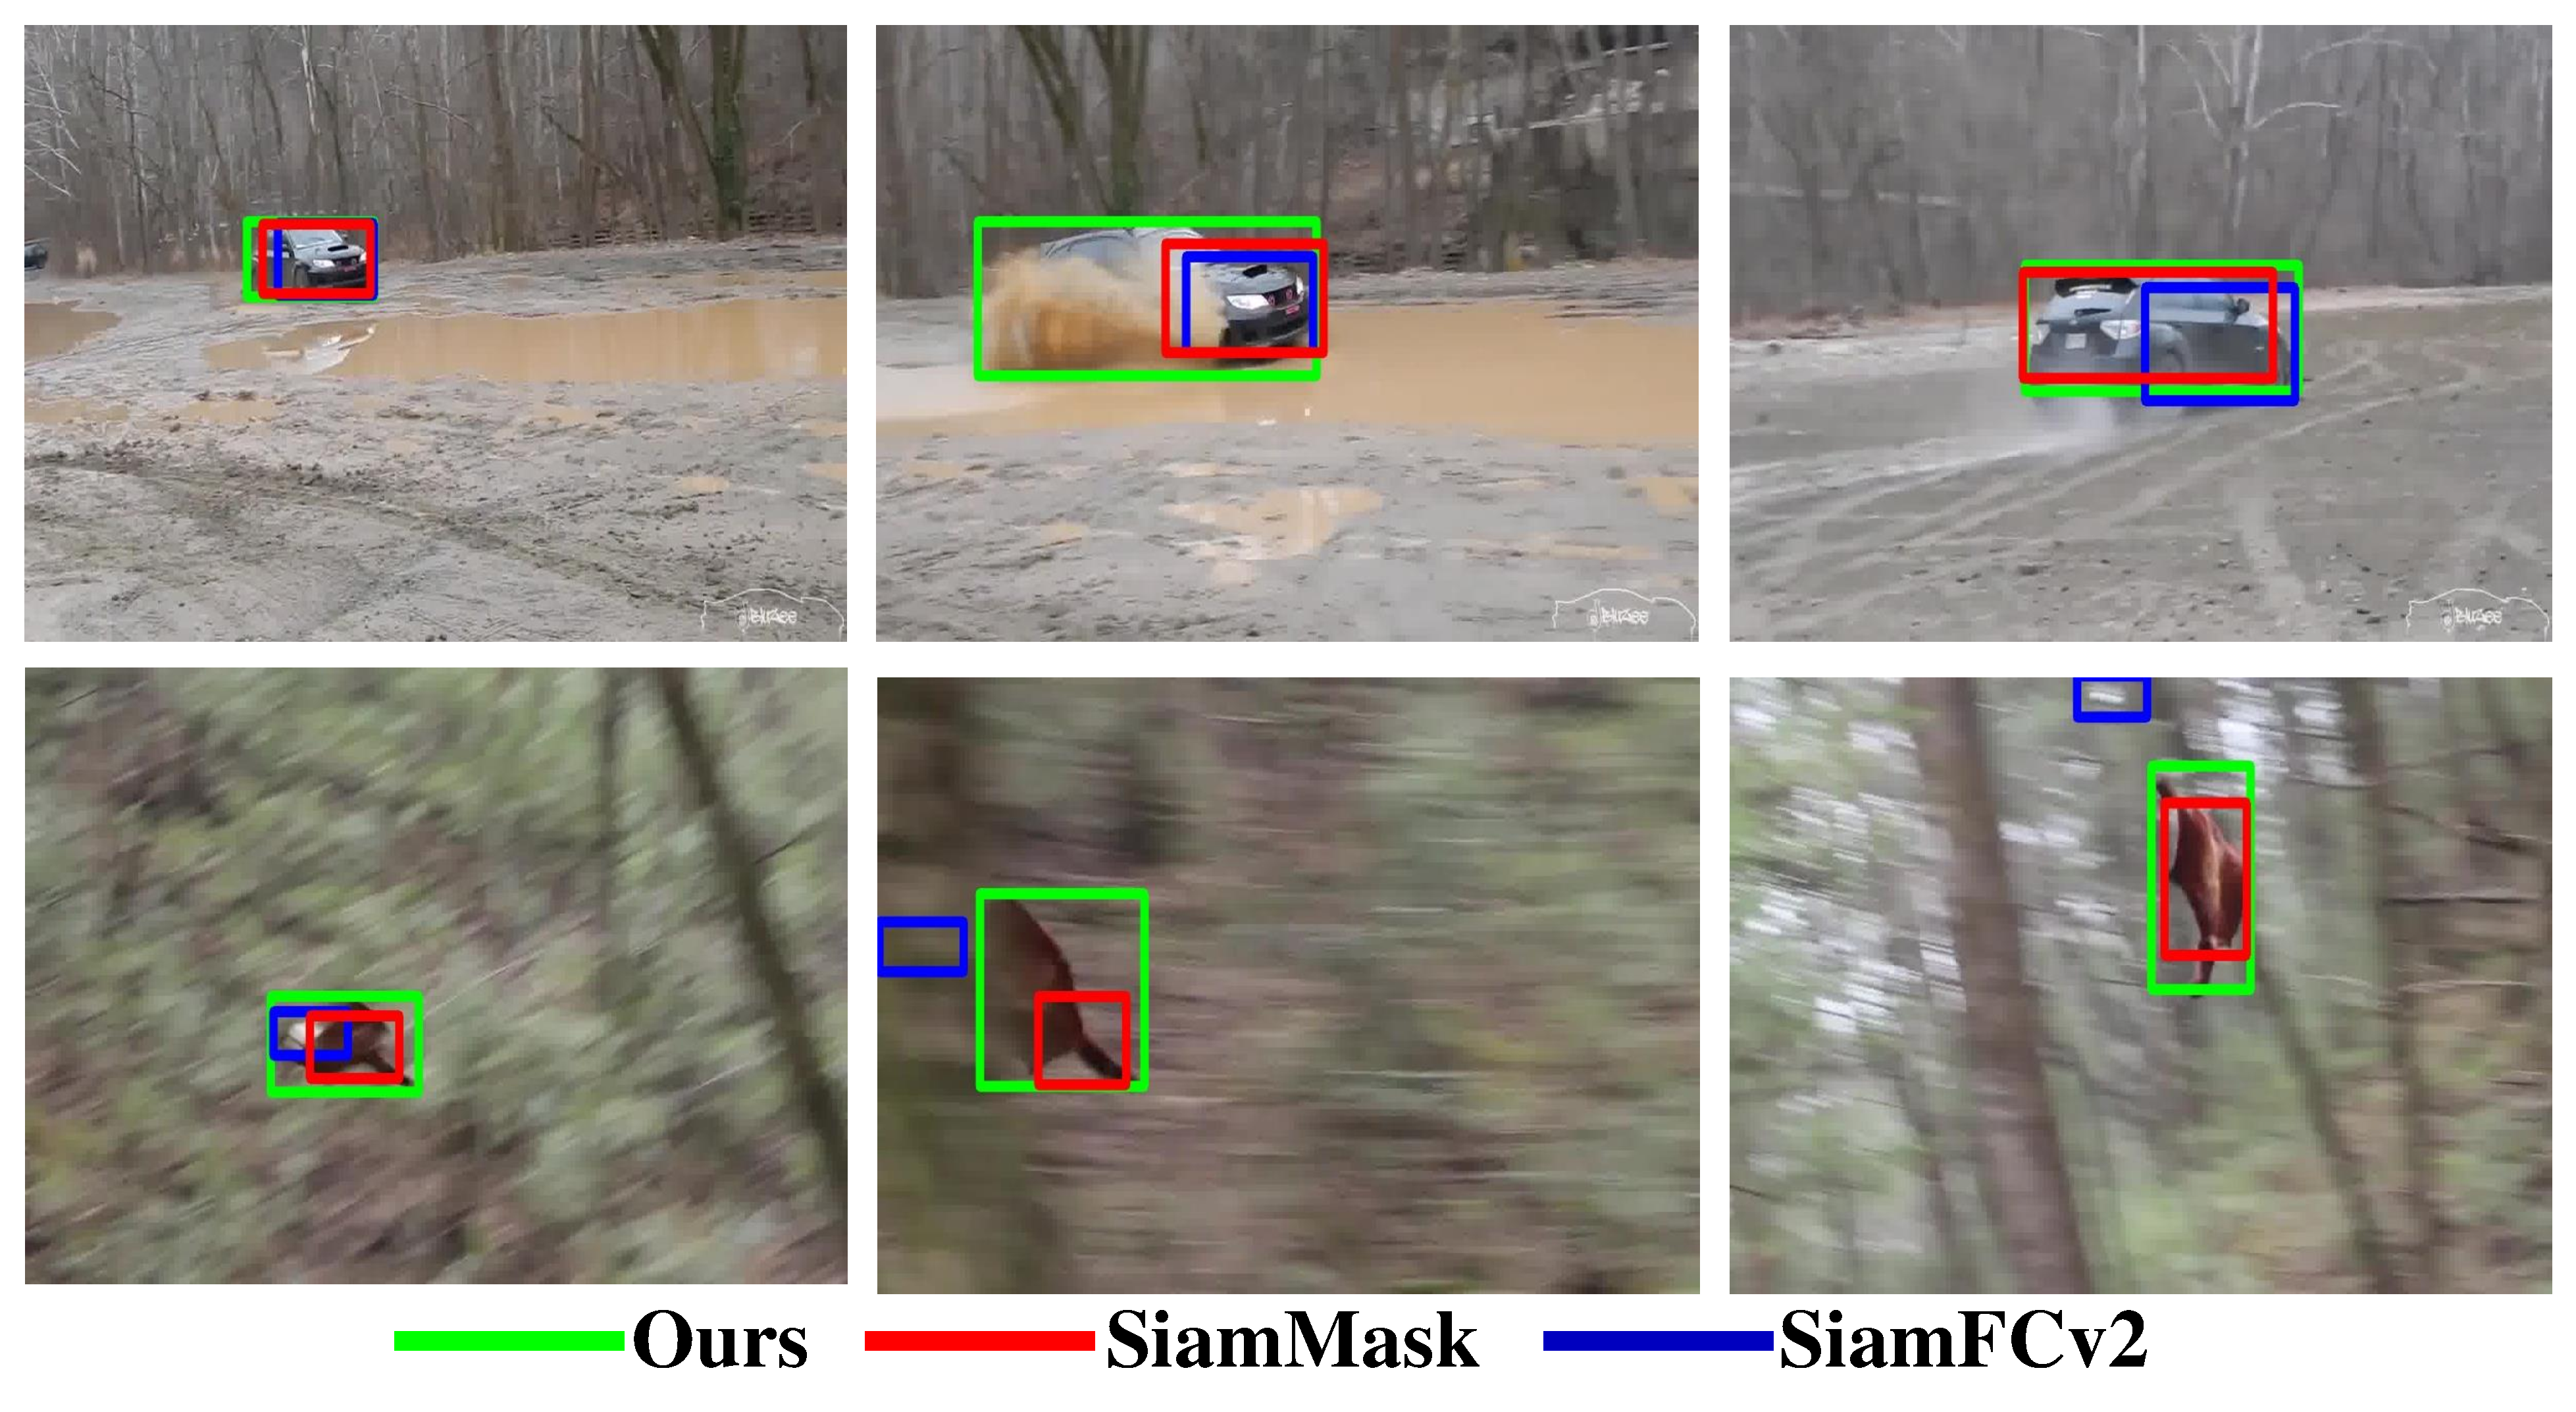
\includegraphics[width=0.95\textwidth]{Img/end/visulization.pdf}
    \caption{本章提出的跟踪器与主流跟踪器 SiamMask \cite{Wang2018SiamMask} 和 SiamFCv2 \cite{SiamFC} 在 GOT-10k \cite{GOT-10k} 测试集上的跟踪结果对比展示。本章提出的方法可有效处理不良的目标表观。}
    \label{fig:end_vis}
\end{figure}

本章提出的时间信息增强的跟踪算法提高了基于孪生网络的视觉目标跟踪器的特征表示能力,从而提高了跟踪鲁棒性与准确性。同时,在对抗性 Dropout 模块的引导下学习对于退化的目标表观具有判别能力的特征,通过端到端的网络离线训练使得整个孪生网络跟踪算法的跟踪性能得到大幅度提升。本章在视觉目标跟踪数据集 GOT-10k \cite{GOT-10k} 和 UAV20L \cite{mueller2016benchmark} 上验证了方法的有效性并与当前最好的跟踪算法进行了比较。
\subsection{实验设置}

\begin{figure}[t]
    \centering
    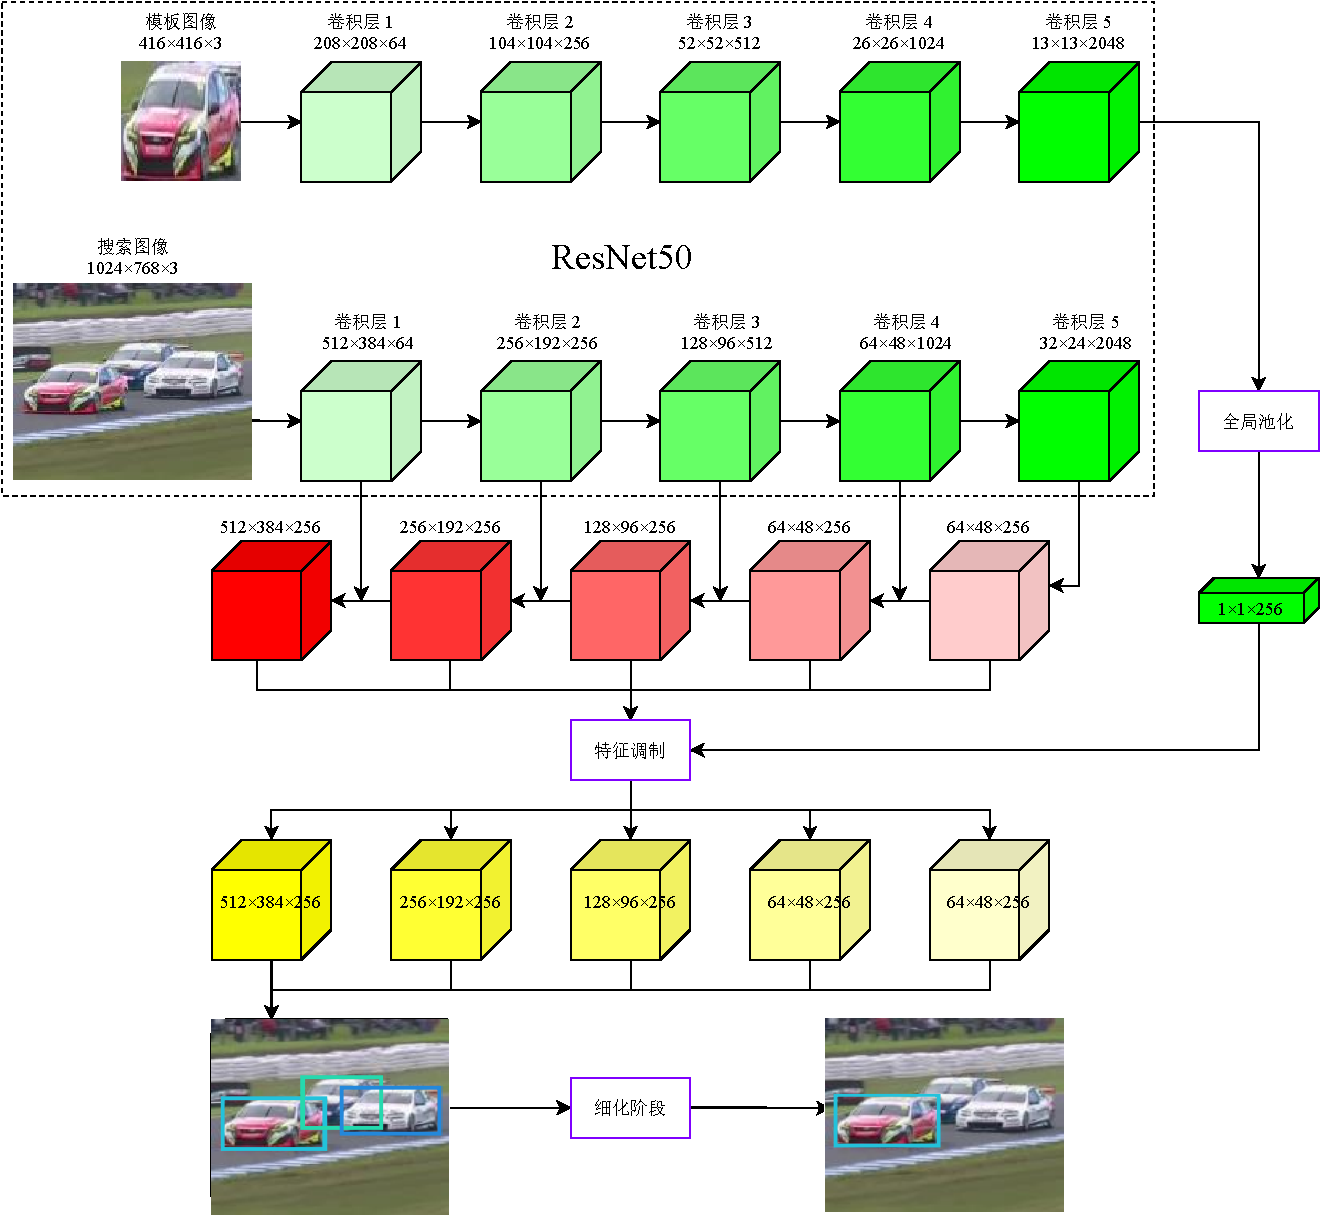
\includegraphics[width=1.0\textwidth]{Img/end/FPN.pdf}
    \caption{本章提出的跟踪框架的网络结构参数展示。}
    \label{fig:end_FPN}
\end{figure}

\textbf{网络架构设计}:本章提出的时间信息增强的孪生视觉目标跟踪网络主要由三个子网络组成,分别是用于共享特征提取的主干网络、用于生成特定目标特征的特征调制子网络以及用于边框微调的区域细化子网络。它们的网络结构如图 \ref{fig:end_FPN} 所示,主干网络为基于 ResNet50 的特征金字塔网络,可以为搜索区域图像提取不同分辨率的特征图,以提升特征表示能力。

\nopagebreak[3]
\begin{figure}[!t]
    \centering
    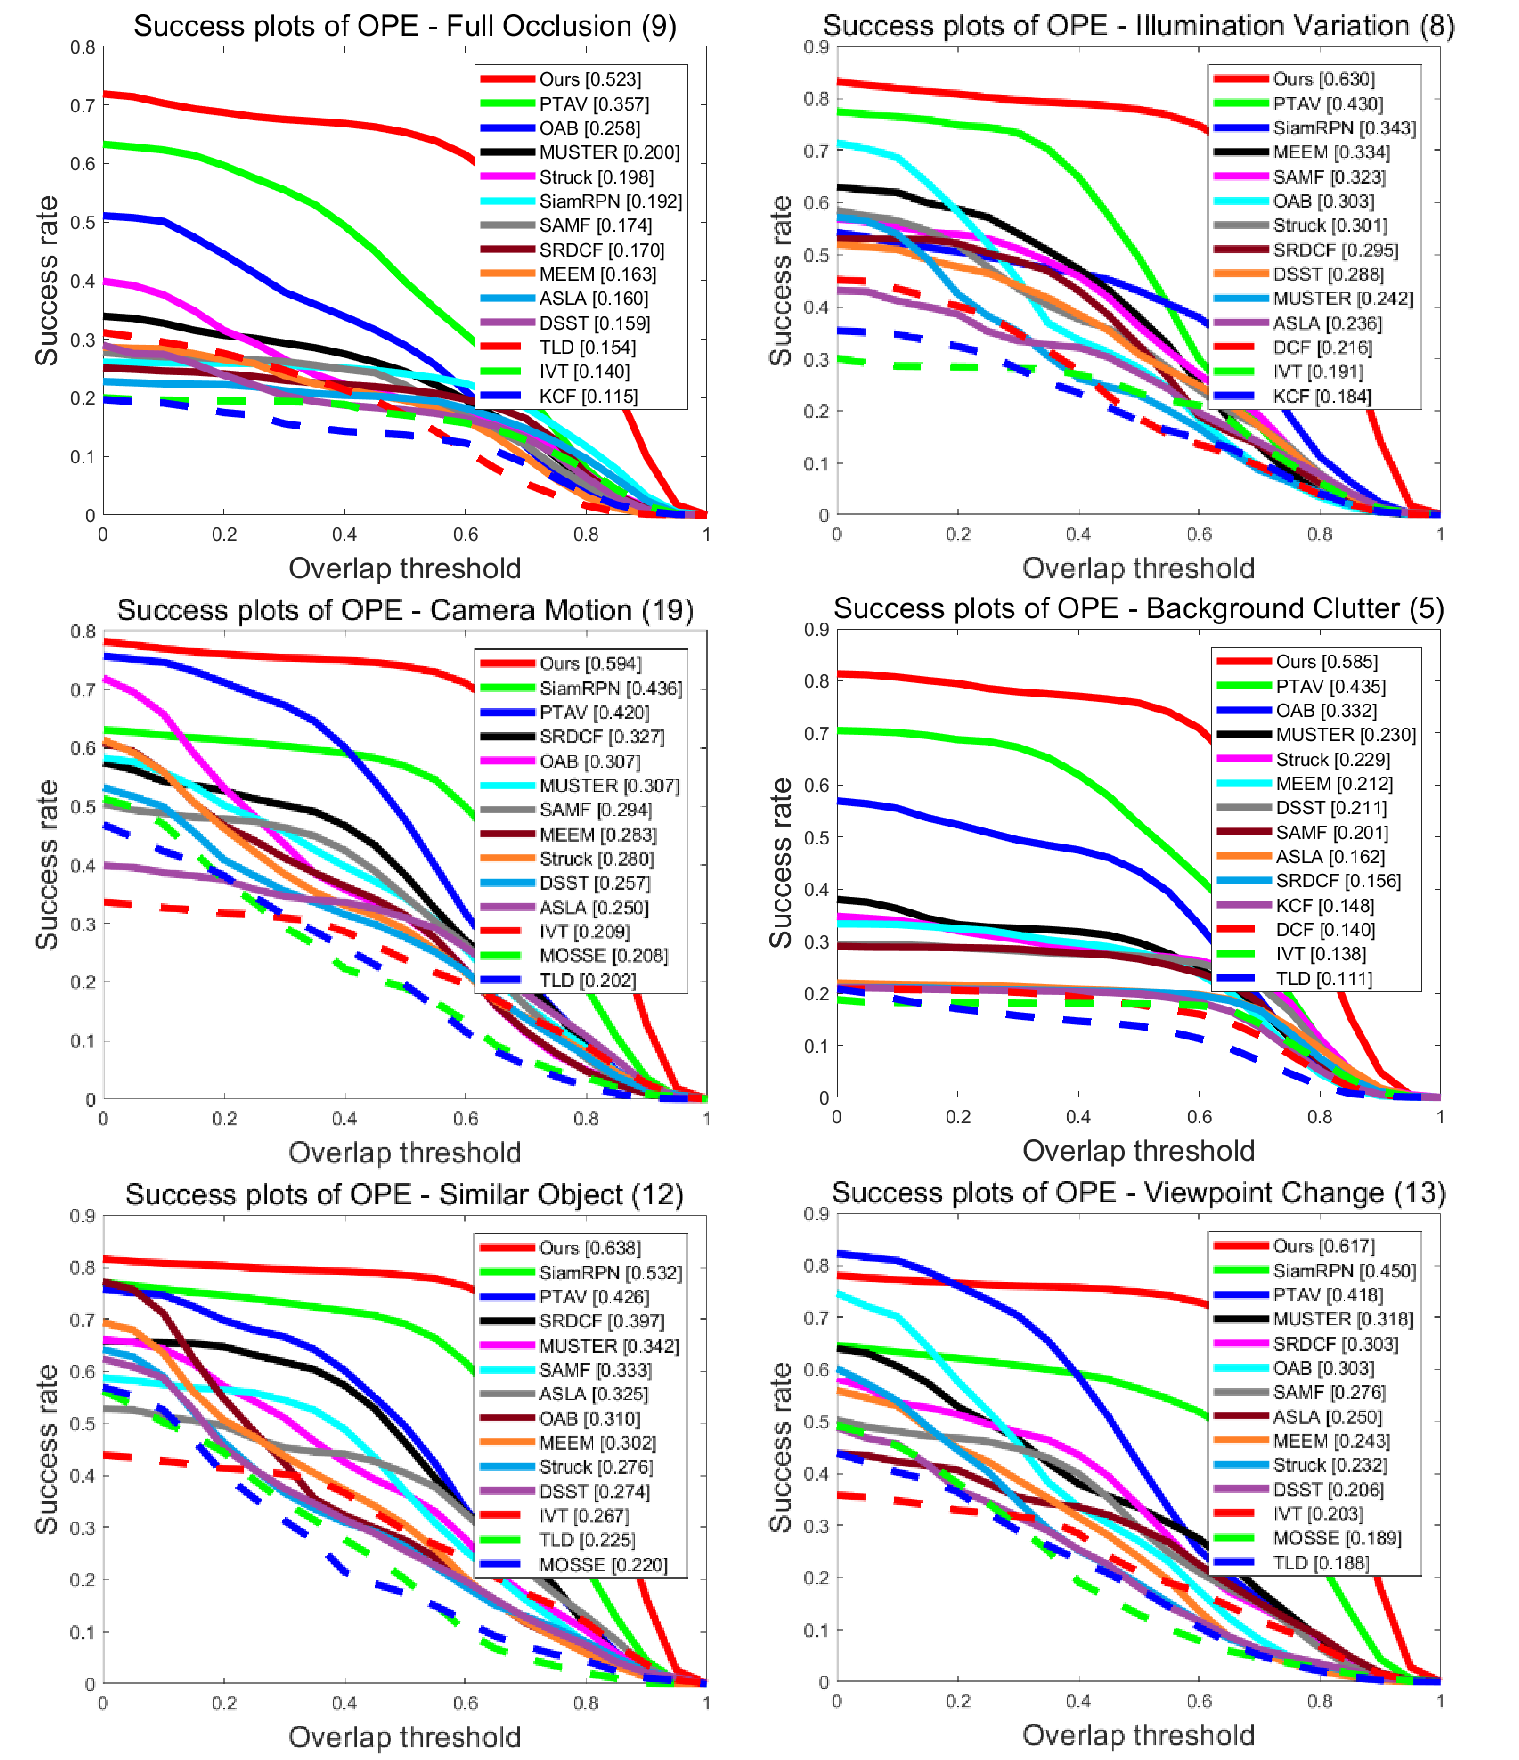
\includegraphics[width=1.0\textwidth]{Img/end/UAV20L_1.pdf}
    \caption{基于评测库 UAV20L \cite{mueller2016benchmark} 的 6 个属性标注的算法跟踪性能对比展示。}
    \label{fig:end_uav20l_attr_1}
\end{figure}
\nopagebreak[3]
\begin{figure*}[t!]
    \centering
    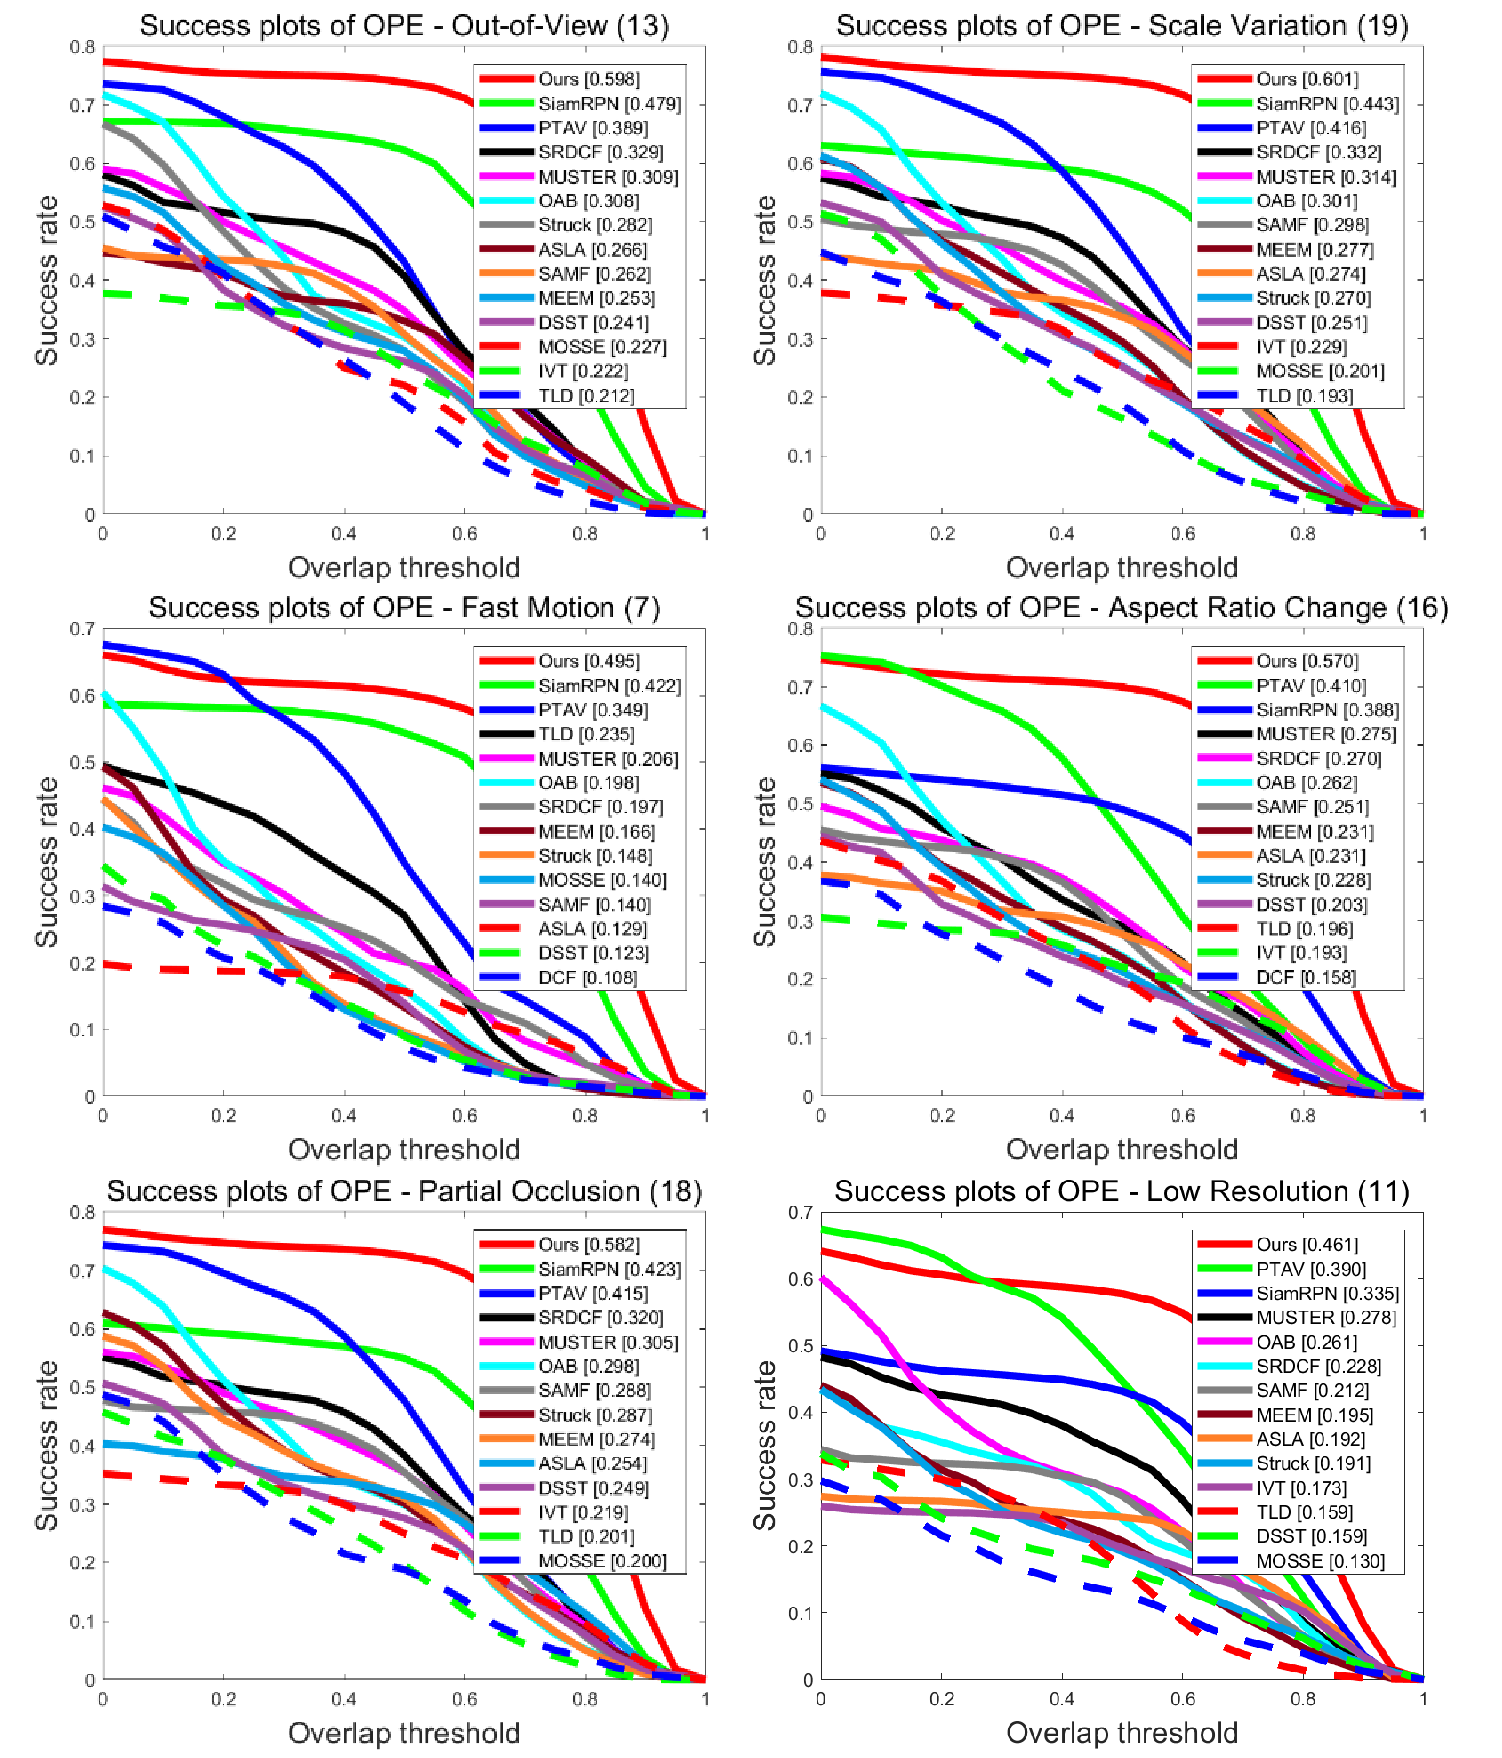
\includegraphics[width=1.0\textwidth]{Img/end/UAV20L_2.pdf}
    \caption{基于评测库 UAV20L \cite{mueller2016benchmark} 的 6 个属性标注的算法跟踪性能对比展示。}
    \label{fig:end_uav20l_attr_2}
\end{figure*}

\textbf{训练数据}:为了提高特征表示的泛化能力和判别能力,同时避免在稀缺的跟踪数据上过拟合,离线训练过程在大规模单目标视频跟踪数据库 GOT-10k \cite{GOT-10k} 的训练数据集中训练网络参数。该数据集包含超过 10000 个视频序列,具有较为丰富多样的视频场景分布。该数据集被广泛应用在最近提出的孪生网络跟踪算法 \cite{SiamFC++} 的训练中。

\textbf{优化器参数设定}:本章使用动量为 0.9 的随机梯度下降(stochastic gradient descent,SGD)优化器从在 ImageNet 上预训练的网络参数开始训练,并将权值衰减参数设置为 0.0005。该模型经过 90000 次迭代训练,学习率从 $10^{-2}$ 指数衰减到 $10^{-4}$。

本章所提出的时间信息增强的孪生网络跟踪器使用 Pytorch 在 Python 中实现,所有实验在装配有 Intel(R) Xeon(R) CPU E5-2630 v4 @ 2.20GHz 和 NVIDIA TITAN 1080Ti GPU 的工作站上执行。

\subsection{基于数据集 GOT-10k 的评测结果分析}
\begin{table}[t]
\centering
\caption{本章提出的跟踪算法与相关算法在 GOT-10k \cite{GOT-10k} 测试集上的评测结果。}
\begin{tabular}{l l l l}
\bottomrule
跟踪器   &  AO   &  $\textbf{SR}_{0.50}$ & $\textbf{SR}_{0.75}$  \\
\hline
本章算法 &  $\textbf{0.577}^\textbf{1}$ & $\textbf{0.662}^\textbf{1}$  & $\textbf{0.509}^\textbf{1}$  \\
SiamMask \cite{Wang2018SiamMask} &  0.459&  0.560 &0.205 \\
SiamFCv2 \cite{valmadre2017end} &  0.374&  0.404 &0.144 \\
SiamFC \cite{SiamFC}  &  0.348&  0.353 &0.098 \\
GOTURN \cite{GOTURN} &  0.347&  0.375 &0.124 \\
CCOT	 \cite{danelljan2016beyond} &  0.325&  0.328 &0.107 \\
ECO \cite{danelljan2017eco} &  0.316&  0.309 &0.111 \\
CF2 \cite{CF2} &  0.315&  0.297 &0.088 \\
MDNet \cite{MDNet} &  0.299&  0.303 &0.099 \\
%CFNetc2	 &  0.293&  0.265 &0.087 \\
%ECOhc	 &  0.286&  0.276 &0.096 \\
\bottomrule
\end{tabular}
\label{table:end_got10k}
\end{table}
本节在 GOT-10k \cite{GOT-10k} 数据集上评估本章提出的算法。
GOT-10k 是最近提出的目标跟踪数据集,包含超过 10000 个视频序列,目标由矩形边界框注释。
GOT-10k 测试集包括 180 段视频序列,具有 84 种不同的目标类别和 32 种运动模式,并使用文献 \cite{GOT-10k} 中提出的平均重叠(AO)分数和成功率(SR)作为性能指标。AO 表示所有真实边界框和估计边界框之间重叠的平均值,而 SR 表示重叠超过 0.5/0.75 的成功跟踪帧的百分比。

\textbf{创新点有效性验证}
为了分析本章提出的时间聚合模块和对抗性 Dropout 模块的有效性,本组实验训练了两个跟踪网络的变体。变体 1(参见表 \ref{table:end_ablition} 第一行)在本章最终提出的跟踪器中同时剔除了时间聚合模块和对抗性 Dropout 模块。变体 2(参见表 \ref{table:end_ablition} 第二行)在本章最终提出的跟踪器中剔除对抗性 Dropout 模块,仅保留时间聚合模块。表 \ref{table:end_ablition} 的第三行表示本章最终提出的跟踪器,同时配备有时间聚合模块和对抗性 Dropout 模块。
本组实验在 GOT-10k 测试集上对上述三个跟踪器的性能进行了对比。
从第一行可以看出,变体 1 的 AO 值为 0.542,具有较好的跟踪性能。这是因为主干网络采用了特征金字塔网络,可充分利用目标的底层和高层信息,对于大目标在较高尺度上进行预测,对于小目标在较低尺度上进行预测,从而提高了跟踪性能。然而,该跟踪器仅利用单帧图像进行跟踪,未利用视频中的时间信息,因此当目标表观发生退化时具有较差的性能。
从第二行可以看出,变体 2 的 AO 值为 0.561,相比于变体 1,AO 性能提高了 1.9%。
这是因为时间聚合模块通过聚合来自相邻帧的时间信息以改善每帧特征。
从第三行中可以看出,通过添加对抗性 Dropout 模块,跟踪器的 AO 进一步增加了 1.6%。
这是因为对抗性 Dropout 模块提高了本章提出的孪生跟踪网络的特征判别能力。

\textbf{与其他跟踪算法的比较}
本组实验将本章提出的方法与多个主流跟踪器进行了比较。
表 \ref{table:end_got10k} 和图 \ref{fig:end_got10k} 中显示了这些跟踪器的性能。
与所对比的方法相比,本章提出的方法实现了 0.577 的 AO 值。

ECO \cite{danelljan2017eco} 是基于 DCF 的最新跟踪器,它引入了分解卷积运算符,可显著减少 DCF 模型中的参数数量。相比之下,本章提出的跟踪器基于强大的孪生架构。因此,本章提出的跟踪器的 AO 得分明显优于 ECO,提高了 26.1%,这表明了孪生体系结构在目标跟踪任务方面的有效性。
SiamMask \cite{Wang2018SiamMask} 是最近提出的孪生跟踪器。它同时在三个任务上训练一个孪生网络,每个任务都对应一种不同的策略,以建立真实目标和候选区域之间的对应关系。
然而,SiamMask 是基于局部搜索机制的:在以上一帧的目标位置为中心的小邻域内搜索目标,且未充分利用时间信息。相比之下,本章提出的跟踪算法使用全局搜索机制,始终能够感知整个图像上的目标,且能充分利用时间信息。因此,本章提出的跟踪器的 AO 得分高出 SiamMask 11.8%,这体现了时间聚合模块的有效性。

\subsection{基于数据集 UAV20L 的评测结果分析}
本组实验在 UAV20L \cite{mueller2016benchmark} 长期跟踪数据集中评估跟踪器。
它包含从低空鸟瞰视角捕获的 20 个高清视频序列,平均序列长度为 2934 帧。
在此实验中,使用两种评价指标对跟踪器进行比较:精确度和成功率。精确度表示预测边界框中心与相应的真实边界框中心之间的距离。成功率表示预测边界框与真实边界框的边框重叠。
在图 \ref{fig:end_uav20l} 中可以看出,本章提出的算法具有较好的跟踪性能。
在成功图中,本章提出的跟踪器获得的 AUC 得分为 0.606,
在精度图中,本章提出的跟踪器的得分为 0.804,超过了所列出的其他跟踪算法,例如 SiamRPN \cite{SiamRPN} 和 PTAV \cite{fan2018parallel}。这证明了本章提出的跟踪器在长期跟踪情况下的有效性。

此外,本组实验在 UAV20L 数据集上进行了基于属性的分析(参见图 \ref{fig:end_uav20l_attr_1} 和图 \ref{fig:end_uav20l_attr_2})。UAV20L 包含常见的视觉跟踪挑战。其中,宽高比变化(aspect ratio change,ARC)表示第一帧中目标的宽高比与至少后续一帧中目标宽高比的比值超出区间 $[0.5, 2]$;背景混杂(background clutter,BC)表示目标附近的背景表观与目标表观近似;相机运动(camera motion,CM)表示相机的突然运动;快速运动(fast motion,FM)表示目标标注框在相邻两帧之间的位移超过 20 像素;完全遮挡(full occlusion,FOC)表示目标被完全遮挡;光照变化(illumination variation,IV)表示目标的光照发生显著变化;低分辨率(low resolution,LR)表示至少有一个真实标注框的分辨率小于 400 像素;视线外(out-of-view,OV)表示目标的某些部分离开视线;部分遮挡(partial occlusion,POC)表示目标被部分遮挡;相似目标(similar object,SOB)表示目标附近有相似形状或相同类型的目标;尺度变化(scale variation,SV)表示目标的初始边界框和至少一个后续边界框的尺度比率超出范围 $[0.5, 2]$;视点改变(viewpoint change,VC)表示视点会显著影响目标表观。
与所列出的方法相比,本章提出的方法在所有属性下均取得了最好的跟踪结果。
在文献 \cite{fan2018parallel} 中,Fan 等人提出了并行跟踪与验证(parallel tracking and verifying,PTAV)跟踪框架。PTAV 由跟踪器和验证器两个模块组成,在两个单独的线程上并行工作。跟踪器旨在提供实时跟踪预测,在大多数时间表现良好;验证器检查跟踪结果并在必要时校正跟踪结果。通过两个模块的合作,PTAV 既具有较高的跟踪效率,也具有较强的跟踪性能。因此,该算法在光照变化、宽高比变化等属性上得分较高。尽管如此,PTAV 与本文提出的算法仍具有较大差距。比如在光照变化属性中,PTAV 的成功率为 0.430,而本章提出的算法成功率为 0.630。可能的原因是 PTAV 仅基于单帧图像执行跟踪,而本章提出的跟踪器融合了相邻帧中目标的表观信息,更能克服由于光照变化而造成的目标表观退化现象。

\section{本章小结}
本章提出了一种时间信息增强的视觉目标跟踪算法。该算法主要在特征提取方面对基于孪生网络的视觉目标跟踪算法进行优化。首先,从基于孪生网络的在线视频跟踪算法鲁棒性不足问题出发,将时间信息引入在线视觉目标跟踪中。通过来自相邻帧的目标表观信息的聚合,使得目标表观特征更加丰富,弥补基于孪生网络的视觉目标跟踪算法局限于从单帧提取目标表观,对目标表观表示能力不足的缺点,从而提高跟踪的效果,实现鲁棒的跟踪。在端到端时间聚合的基础上,通过引入对抗性 Dropout 模块,并通过在大规模数据集上端到端训练,使得孪生网络跟踪器在目标由于运动模糊等导致的表观不佳的情况下具有更好的表现,从而进一步提高跟踪的鲁棒性。本章在目前流行的视觉目标跟踪评测库上进行了算法的对比实验以及成分分析实验,从而验证算法改进的有效性。